\subsection{Konzentrationsabhängigkeit von Schichtdicken}

Hier wird nun die Konzentrationsabhängigkeit von den Schichtdicken untersucht. Dafür werden, ähnlich wie in der vorherigen Aufgabe, die ermittelten Schichtdicken für beide Messmethoden gegen die Konzentration geplottet, siehe Abb.~\ref{fig:concentration}. Ebenso wird wieder ein Fit gemäß Gl.~\eqref{eq:schubert} durchgeführt, welcher für $\omega = const.$ zu einer linearen Abhängkeit der Schichtdicken von der Konzentration führt. Wichtig zu beachten ist hierbei, dass es zu einem Regimewechsel in dem von uns betrachteten Konzentrationsbereich kommt: ab einer bestimmten kritischen Konzentration $c_0$ der Polystyrollösung ändert sich die Steigung der Geraden, weshalb hier mit 2 verschiedenen Fits gearbeitet wird. Der Steigungswechsel lässt sich durch die sich verändernde Viskosität der Lösung erklären, da die Polymerketten anfangen zu überlappen~\cite[]{Daum}. 

\begin{figure}
    \centering
    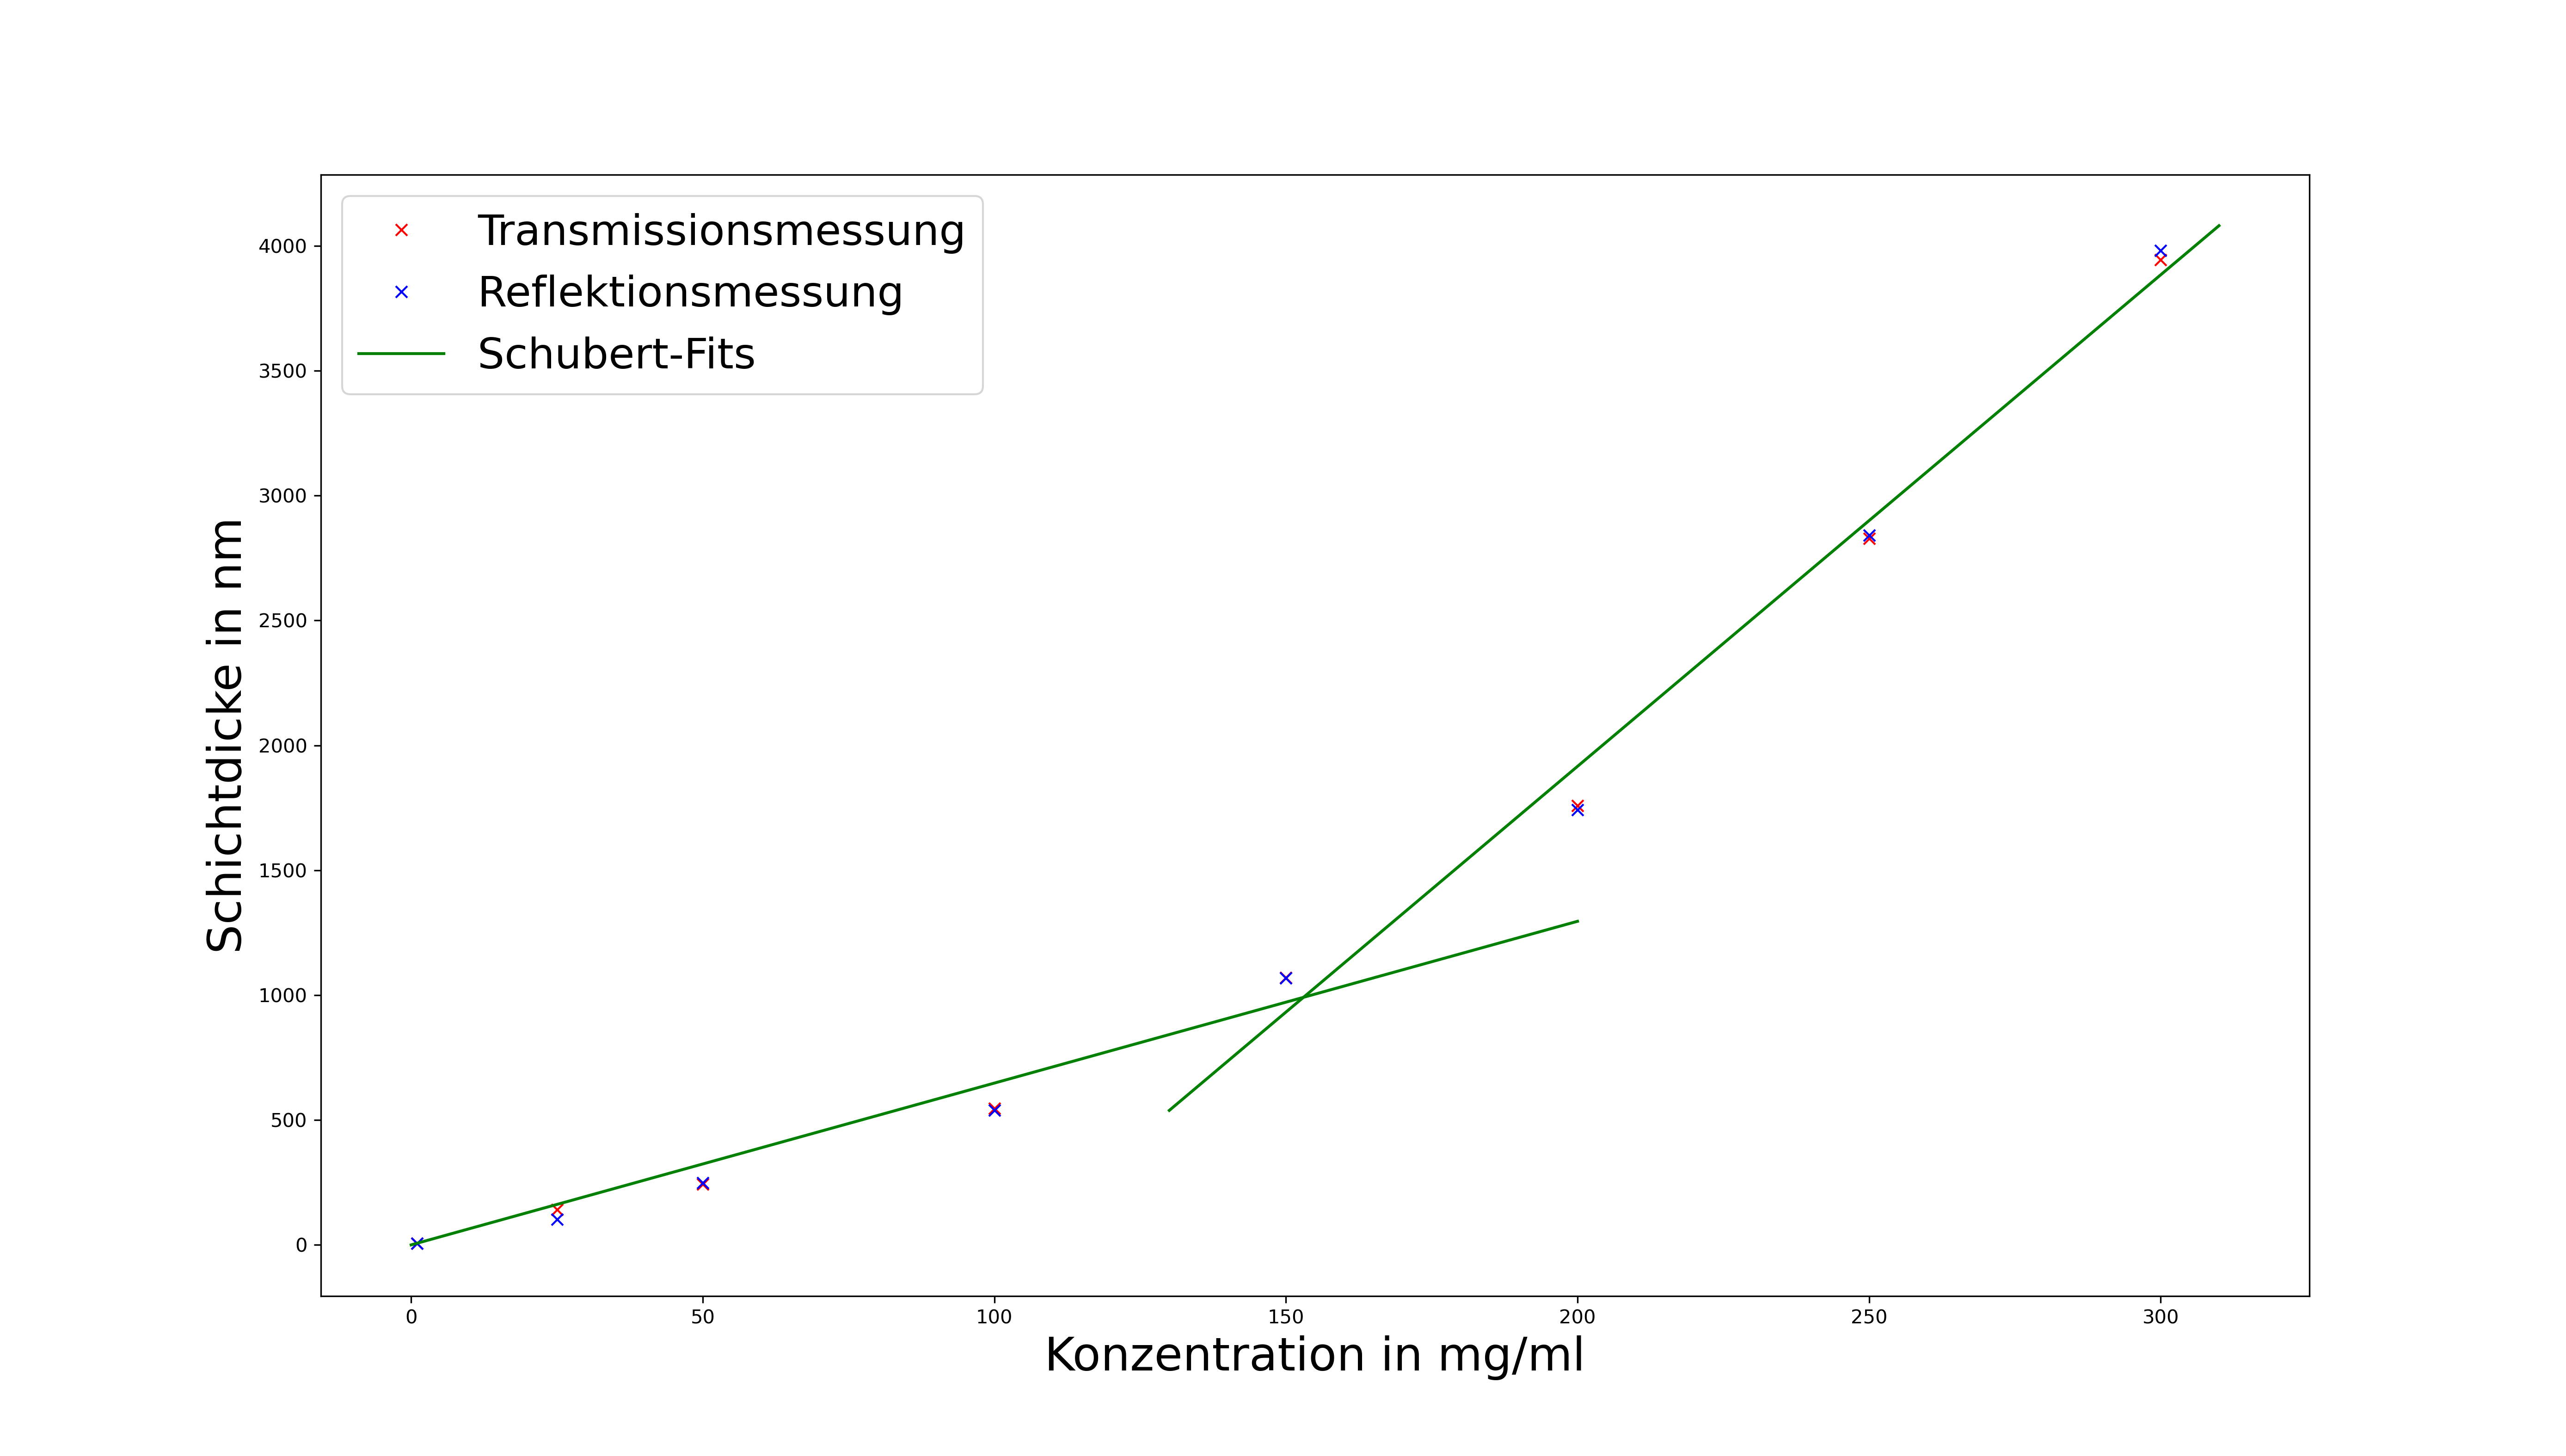
\includegraphics[width=\linewidth]{schubert_conc.png}
    \caption{Reflektions- und Transmissionsmessungen der Schichtdicken in Abhängigkeit der Konzentration der Polystyrollösung mit zusätzlichen Fits nach der Schubert-Gleichung.}
    \label{fig:concentration}
\end{figure}

Die kritische Konzentration ergibt sich aus dem Schnittpunkt der beiden Geraden zu 
\begin{equation*}
    c_0 = \SI{153}{\milli\gram\per\milli\litre}
\end{equation*}

Nun soll die root-mean-sqaure end-to-end distance $R_{rms}$ gemäß~\cite[]{properties} für Polystyrol berechnet werden. Diese ergibt sich folgendermaßen:
\begin{equation}\label{eq:rms}
    R_{rms, 1} = \sqrt{C_\infty n l^2}
\end{equation}
mit $C_\infty = 9,5$ dem charakteristischen Flory-Verhältnis für Polystyrol und $l = \SI{1,54}{\angstrom}$ der Länge der Rückgratbildung~\cite[]{Anleitung}. $n$ ist die Anzahl der Bindungen im Polymerrückgrat, welche folgendermaßen berechnet wird:
\begin{equation}
    n = \frac{M_W}{M_N}
\end{equation}
mit $M_W = \SI{35000}{\gram\per\mol}$ der molaren Masse des hier verwendeten Polystyrols und $M_N = \SI{104,15}{\gram\per\mol}$ der molaren Masse einer einzelnen $\mathrm{C}_8\mathrm{H}_8$-Einheit des Polystyrols~\cite[]{properties}. Hiermit ergibt sich $n \approx \num{336}$ und schließlich
\begin{equation*}
    R_{rms, 1} = \SI{87,0}{\angstrom}
\end{equation*}
Für unsere Polystyrollösung soll diese Größe nun zusätzlich gemäß~\cite[]{Daum} berechnet werden. Hier gilt:

\begin{equation}
    R_{rms, 2} = \num{2,84e-8} \cdot \left(\frac{M_W}{c_o}\right)^\frac{1}{3}
\end{equation}
mit $M_W$ wieder der molaren Masse unserer Polystyrols und $c_0$ der vorher ermittelten kritischen Konzentration. Hiermit ergibt sich:
\begin{equation*}
    R_{rms, 2} = \SI{173,7}{\angstrom}
\end{equation*}

Beide Ergebnisse liegen zwar in der selben Größenordnung, unterscheiden sich jedoch deutlich. Möglicherweise ist der zweite Ansatz keine gute Näherung für unsere Polystyrollösung.

Abschließend sollen die drei verschiedene Polymer-Modelle \textit{random coil, womlike chain} und \textit{rodlike} anhand von Rechnungen vgl.~\cite[]{regimes} dahingehend bewertet werden, zu welchem unsere Polystyrollösung am ehesten passt. 

Im \textit{random coil} Modell berechnet sich die kritische Überlappkonzentration folgendermaßen:
\begin{equation}
    c_{RC} = \frac{M_W}{N_A \left(\nicefrac{R_{rms}}{2}\right)^3} = \SI{705,7}{\milli\gram\per\milli\litre}
\end{equation}
mit $N_A$ der Avogrado-Konstante und $R_{rms}$ aus Gl.~\ref{eq:rms}.
Im \textit{wormlike chain} Modell ergibt sich die kritische Überlappkonzentration zu:
\begin{equation}
    c_{WL} = 2^\frac{3}{2} \frac{M_W}{N_A \left(\rho n l\right)^\frac{3}{2}} = \SI{441,5}{\milli\gram\per\milli\litre}
\end{equation}
mit $\rho = \SI{10}{\angstrom}$ der Persistenzlänge von Polystyrol aus~\cite{density}.
Für das \textit{rodlike} Modell lässt sich für die kritische Überlappkonzentration folgender Wert berechnen:
\begin{equation}
    c_{RL} = 2^\frac{3}{2} \frac{M_W}{N_A \left(nl\right)^3} = \SI{1,19}{\milli\gram\per\milli\litre}
\end{equation}
Beim Vergleich der 3 verschiedenen Werte mit unserem gemessenen Wert für die Überlappkonzentration fällt auf, dass kein Wert gut passt. Am ehesten lässt er sich noch mit dem Wert aus dem \textit{wormlike chain} Modell vergleichen, jedoch ist auch dieser Wert noch deutlich zu hoch. Polystyrol scheint ein halbflexibles Polymer zu sein. Die einzelnen Segmente sind steif, wobei aufeinander folgende Segmente in ungefähr die selbe Richtung zeigen~\cite[]{regimes}. 
Der große Unterschied zwischen unserem und dem berechneten Wert könnte neben klassischen Fehler und der Tatsache, dass der Wert für $\rho$ selber nur eine theoretische Abchätzung in~\cite{density} ist, auch daran liegen, dass das Modell nicht vollständig mit unserem verwendeten Polystyrol übereinstimmt.